\chapter{ISBI Challenge 2013}
\section{Introduction}
The goal of the ISBI Challenge, as announced on their website (\cite{challenge}), is to give an overview and understanding of availible algorithms for single particle localization microscopy. The focus was on 2d localisation, to give information about the depth of a localisated spot was optional. To benchmark results one needs groundtruth. Therefore the organizers created synthetic datasets of biologically relevant structures such as tubulins. To match realistic conditions the data was transformed to contain different kinds of noise and background.\newline
The participants were given training data sets and the corresponding groundtruth. One month before the deadline of the challenge the test sets were released. There were two different kinds of datasets in principle. One with very dense spots and shorter sequences, the other with longer sequences and fewer spots per frame.\newline
All paricipants were asked to submit their results and also the time it took to run the algorithm and the hardware configuration of the used system.

\section{Terminology}
To be able to compare different algorithms there must be a way to determine the correctly detected spots. To do so for each estimated positon of a fluorophor, the nearest correct position of the molecule in the groundtruth data was searched within a lateral tolerance disc. Once a match was found this two spots were taken out of consideration for the matching.\newline
One important parameter for this evaluation is the radius of the lateral tolerance disk, because it has great influence on the number of detections considered to be true positives (TP).\newline
Detections with no associated spot in the groundtruth are called false positives (FP), spots in the groundtruth with no matching detection are called false negatives (FN).\newline
This matching is done frame by frame, it is not possible to match a point from different frames even if the $x$ and $y$ coordinates match perfectly but the frame differs.\newline
The precision ($p$) of a classification task is defined as the ration between the number of true positives and the sum of true positives and false positives:
\begin{equation}
\text{precision: }p = \frac{\text{TP}}{\text{TP}+\text{FP}} 
\end{equation}
It is a number between 0 at worst and 1 at best, telling how reliable the result is, how likely it is that a labeld sample really belongs to the predicted class. In this context it means how certain a detected spot has its origin in a fluorophore attached to the investigated structure and it's origin is not wrongly detected background noise.\newline
An other important value is the recall $r$ that is defined as the ratio of true positives and the sum of true positives and false negatives:
\begin{equation}
\text{recall: }r = \frac{\text{TP}}{\text{TP}+\text{FN}}
\end{equation}
The recall lies also in a range from 0 to 1  and gives an impression on how many relevant spots were found.

\section{Measures} 
For the evaluation three different measures were used. The f-score index $f$, the Jaccard index $J$ and the root-mean square distance RSME. 
\subsection{F-score}
The f-score $f$ is directly computed from precision and recall.
\begin{eqnarray}
	\text{f-score: }f &=\frac{2\cdot p \cdot r}{p+r} 
\end{eqnarray}
It ranges from zero for bad performance up to one for perfect results.
\subsection{Jaccard index}
Let $A$ be the set of points of the groundtruth and $B$ be the set of detected points. The Jaccard index $J$ is then defined as:
\begin{equation}
\text{Jaccard: }J = \frac{\left|A\cap B\right|}{\left|A\cup B\right|}
\end{equation}
The intersection is done frame by frame. This means two spots from the groundtruth and the detection set just match if they occure in the same frame. 
\subsection{RSME}
The root-mean square distance gives an impression on how big the squared distance between a spot in the groundtruth and an associated detection was in average. It can be calculated as follows:
\begin{equation}
\text{RSME} = \frac{1}{\left|A\cap B\right|}\sum\limits_{i=1}^{\left|A\cap B\right|} \left(p_a(x,y)-p_b(x,y)\right)^2
\end{equation}
\section{Training data}
All pictures shown in this section are reconstructed from original images or original images as provided by the \cite{challenge}.
\subsection{Bundled tubes datasets}
There were two kinds of bundled tubes data sets, both created from the same underlying structure. One set with a high spot density and a short sequence of 360 frames, the other with fewer spots per frame but 12000 frames in total. Picture \ref{bundledtubesHighowDensityFrame} shows one frame of each data set.\newline
\begin{figure}
\begin{minipage}[t]{0.60\textwidth}
\subfloat[High spot density]{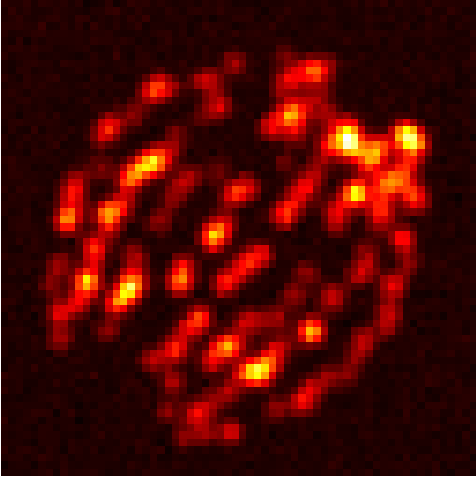
\includegraphics[width = 0.485\textwidth]{pictures/bundledTubesHighDensityFrameFarbig.png}}\hfill
\subfloat[Low spot density]{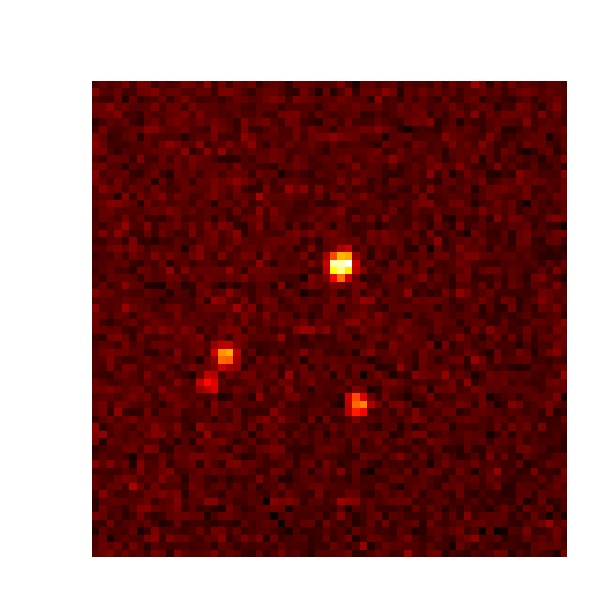
\includegraphics[width = 0.485\textwidth]{pictures/bundledTubesLowDensityFrameFarbig.png}}
	\caption{One frame from bundled tubes training data set}
	\label{bundledtubesHighowDensityFrame}	
\end{minipage}\hfill
\begin{minipage}[t]{0.33\textwidth}
\centering
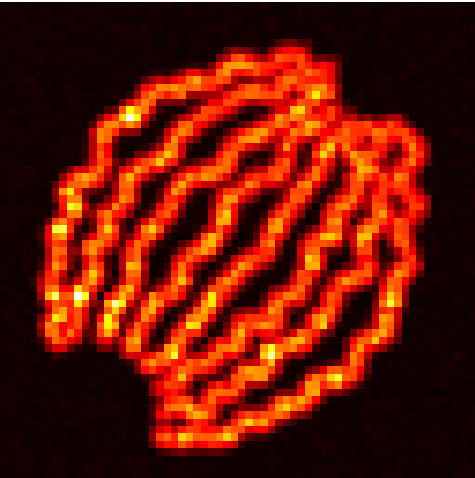
\includegraphics[width = 0.88\textwidth]{pictures/maximumProjectionBundledTubesLSFarbig.png}
	\caption{Maximum projection of bundled tubes data set}
	\label{pctMaximumProjBundledTubes}

\end{minipage}
\end{figure}
The original images were very small, just 64 pixels in each dimension. Both sequences had spatial and temporal constant background. Picture \ref{pctMaximumProjBundledTubes} shows the maximum projection of the bundled tubes data set. The maximum projection is used to reduce the dimensionality of a data set. In this case for each pixel in $x$- and $y$-dimension, in a three dimensional dataset, the brightes value from all frames is taken. 


\subsection{Tubulin data sets}
The other training data sets models 7 microtubules, a structure that is a long filament up to several micrometers long and with a diameter of about 25 nanometers. The spot density lies somewhere between the high density and the low density of the bundled tubes data sets. These data sets show strong inhomogenity in spatial dimensions and moderate inhomogenity in temporal dimension, see Figure \ref{tubulinVariableBg}. This is the reason why in the lower left corner of the maximum projection in Figure \ref{pctMaximumProjTubulin} a brighter area can be seen.

\begin{figure}
\subfloat[Tubulin2 frame 10]{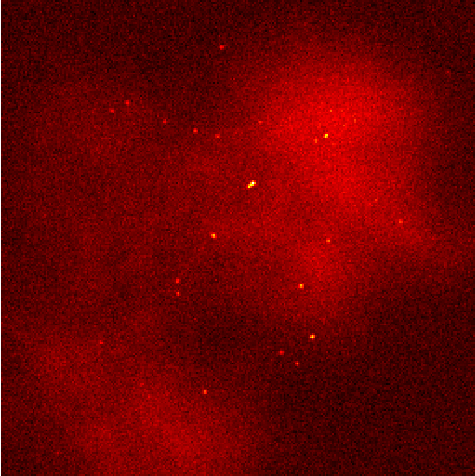
\includegraphics[width = 0.485\textwidth]{pictures/Tubulin2Frame10.png}}\hfill
\subfloat[Tubulin2 frame 1010]{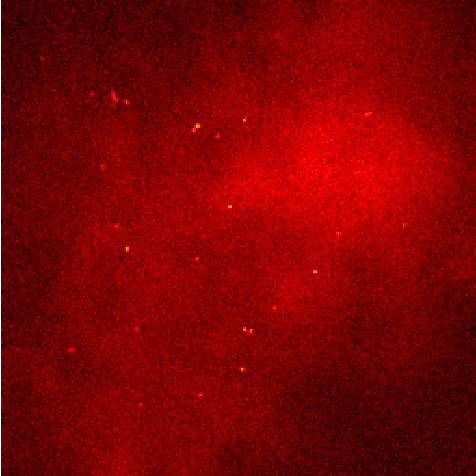
\includegraphics[width = 0.485\textwidth]{pictures/Tubulin2Frame1010.png}}
	\caption{This pictures show the variability of the background in the spatial and temporal dimensions}
	\label{tubulinVariableBg}	
\end{figure}

\begin{figure}
\centering
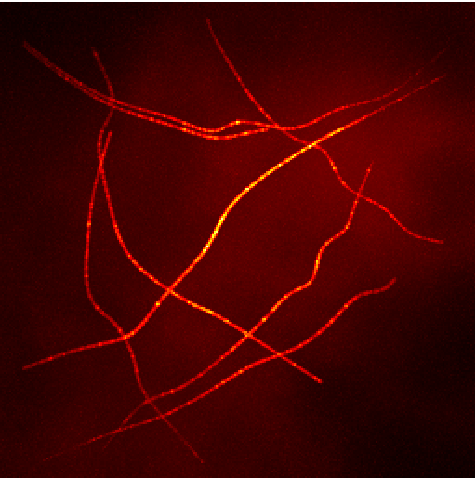
\includegraphics[width = 0.88\textwidth]{pictures/maximumProjectionTubulinFarbig.png}
	\caption{Maximum projection of tubulin data set}
	\label{pctMaximumProjTubulin}


\end{figure}

\section{Submissions}
Now the question arose what it means to be the best algorithm. Is the one the best that finds the most true positives regardles of the number of false positives and the accuracy of detection? Or is it more favorable to find exclusivly correct spots, but less? There are different definitions for the best algorithm possible.\newline
For that reason we run each dataset with three different settings described below. All parameters were set manually.
\subsection{High precision}
A biological question to be answered by STORM microscopy can be: "How are the labeled proteins, distributed over the cell?" There might be just a couple of fluorophors attached to each protein. In that case a high precision is crucial. Otherwise homogenously distributed false positives all over the image might leed to the conclusion that the protein of intest is distributed all over the cell, intead of beeing clustered in some spots.\newline
The high precision submission set the $\alpha$ value to low values to get almost 100 percent precision.
\subsection{High score}
The parameters for the high score submission were set to maximize the Jaccard index. This was done by increasing the $\alpha$ value and estimating the number of true positives and false positives that were found in addition compared to the previously used $\alpha$ value. Based on tests on the trainings date the highest Jaccard index is achieved if the number of new false positives is equal to the number of new true positives. 
\subsection{Highest score via postprocessing}
The higher the $\alpha$ value the more likely it is to detect false positives. But this false positives are distributed all over the image. For the postprocessing the assumption that the true structur in the image shows a higher density of spots than the background with false positives. A mask was created by smoothing the recunstructed image and then thresholding it. This results in a mask that covers image regions with high density. This mask was used to discard all detections which are not covered and therefore are assumed to be false positives in the background.\newline
For the submission a high $\alpha$ was chosen to get also darker true positives. Afterwards the postprocessing was applied. The postprocessing worked well on the contest data because it contained just dense structures. For biological applications the postprocessing has to be used carefully because it discards small, isolated structures, which might be not noise but just widly spread proteins.\newline
Figure \ref{postproc} shows the data before postprocessing, the mask and the result.
\begin{figure}
\subfloat[Image before postprocessing]{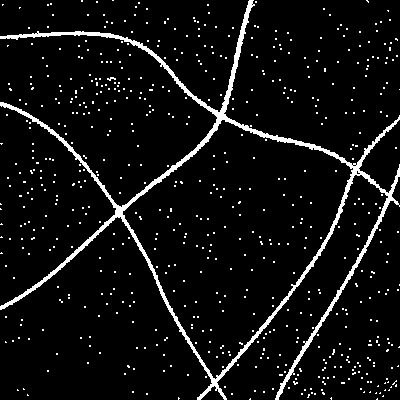
\includegraphics[width = 0.3\textwidth]{pictures/postproc2.png}}\hfill
\subfloat[Mask]{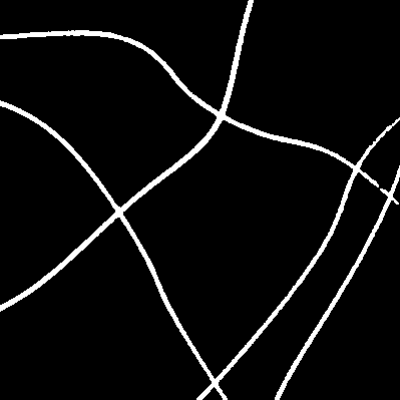
\includegraphics[width = 0.30\textwidth]{pictures/postproc1.png}}\hfill	
\subfloat[Result of postprocessing]{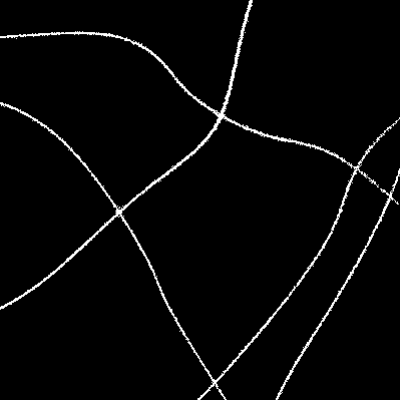
\includegraphics[width = 0.3\textwidth]{pictures/postproc3.png}}

\caption{Overview over the steps of postprocessing.}
\label{postproc}	

\end{figure}


\section{Results}
All tables shown in this section and all diagrams are created from the results released by the \cite{challenge}.
\subsection{High density data}
Table \ref{reshd1}, \ref{reshd2} and \ref{reshd3} show the results of the SimpleSTORM algorithm for the different submissions. The submission with postprocessing applied gave the best results for the Jaccard index, compared to the other two submissions. As expected the settings for high score, but without postprocessing yielded better Jaccard indices than the high precission settings, but also worse precision. As expected the high precision settings resulted in the highest possible precision of one hundred percent. Also the postprocessed data has a perfect precision. This demonstrates that the postprocessing removed the false positives, which decreased the precision in the high score (without postprocessing) results. The accuracy was the same for all three submissions.\newline
The time the software needed was submitted with the results, this means that it depends strongly on the system the algorithms run on. Over all SimpleSTORM took about 90 seconds to process the high density data sets running on an ordinary laptop. This was an average runtime. Most of the faster algorithms used the GPU.

Figures \ref{meanJaccardHighDensity} and \ref{meanRSMEHighDensity} show the mean of the Jaccard index and the RSME score taken over all high density data sets. The results for SimpleSTORM are highlighted. SimpleSTORM achieved an average rank for the Jaccard index and a top five rank for the RSME score. With 100 percent precision it was among 6 other participants on the first rank.




\subsection{Low density data}
The tables \ref{resls1}, \ref{resls2} and \ref{resls3} show the same trends as for the high density data. But with this data sets, the difference between the precisions is greater between the high precision submission and the other two submissions. The runtime was about five minutes. This was, like for the high density data sets, average.



As for the high density data sets the mean scores were calculated for the low density data set and are shown in figure \ref{meanJaccardLowDensity} and \ref{meanRSMEHighDensity}. The results for the precision are also shown in figure \ref{meanPrecisionLowDensity}. SimpleSTORM achieved the third rank in the Jaccard index and intermediate ranks for accuracy and precision.



\subsection{Overall}
Of the 29 participants of the challenge just 15 submitted results for the high density data sets. There is no winner since no software performed well on each score. This can be explained by a trade-off between high accuracy (a low RSME) and the number of spots detected (influence on Jaccard index). For example, bright spots are easier to localize. Just finding the brightest spots yields a good performance on the RSME score but less points. This trade-off can be seen not just in our results, where a high Jaccard index goes along with an intermediate RSME score and vice versa, but also for other algorithms like Fast-ML-HD, which has the highest Jaccard index on the high density data but the second worst RSME score for the same data set.\newline
To compare the different algorithms some metric has to be used that takes the shown trade-off between Jaccard index and accuracy into account. One way is to use the rank each software achieved on the different data sets for different scores and average over it. The results averaging just the mean rank for the Jaccard index and for the RSME score are shown in figure \ref{meanRankLow} for the low density data sets and in figure \ref{meanRankHigh} for the high density data sets.\newline
SimpleSTORM achieves the best mean rank for high density data and the third best result for the low density data sets. \newline
Figure \ref{meanRankOverall} shows the result if the average rank for each data set and for RSME score and the Jaccard index is calculated just based on the ranks of all algorithms that processed both, high density and low density data. All other algorithms were taken out of this consideration. Although this methode of comparison did not weight the ranks which means that extraordinary good performance makes no difference to slightly better performance between two consecutive softwares, but it shows that SimpleSTORM provides a good compromise between many correct detections and high accuracy.



\begin{figure}
\centering
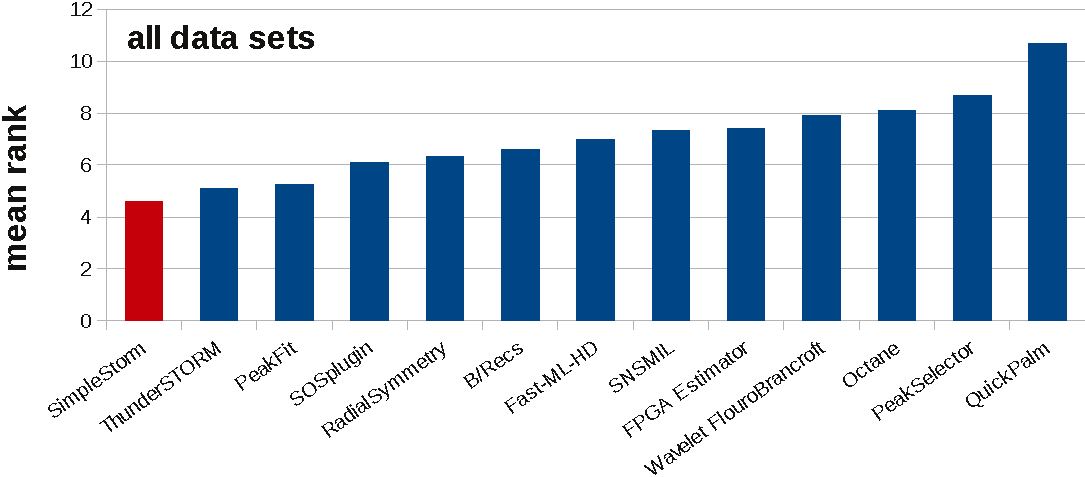
\includegraphics[width = 0.88\textwidth]{pictures/diagrammsChallenge/MeanRankOverallCropped.pdf}
	\caption{Averaged rank over Jaccard index and RSME score for all data sets. Lower ranks are better}
	\label{meanRankOverall}
\end{figure}